\chapter{Medições em Laboratório}

A segunda etapa desta prática consistiu na montagem física dos circuitos projetados e na aquisição empírica dos dados de resposta em frequência. O objetivo primordial desta fase é levantar os valores reais de bancada para o traçado do diagrama de Bode de magnitude e confrontá-los com as previsões matemáticas oriundas da análise teórica, avaliando o impacto prático do efeito de carga e a eficácia do isolamento ativo. Os ensaios foram realizados em 26 de maio de 2026.

\section{Instrumentação e Equipamentos Utilizados}

A confiabilidade das medições experimentais desta prática repousa fundamentalmente na precisão e calibração dos instrumentos de bancada empregados. Todo o procedimento laboratorial de excitação, leitura e diagnóstico dos parâmetros elétricos foi garantido por meio do seguinte \textit{setup} de alto desempenho:

\begin{itemize}
	\item \textbf{Multímetro Digital (True RMS):} Keysight U1253B. Utilizado primariamente para a aferição a frio dos componentes passivos (medição ôhmica e capacitiva) com alta acurácia, atenuando as incertezas paramétricas na posterior análise de dados.
	\item \textbf{Fonte de Tensão Simétrica Contínua:} Keysight E3631A. Responsável pela polarização do amplificador operacional em $\pm 10\text{ V}$, garantindo baixos níveis de \textit{ripple} e ruído de linha acoplado.
	\item \textbf{Osciloscópio Digital (DSO):} Keysight DSO-X 2012A de múltiplos canais. Operado no modo de dois canais simultâneos para o monitoramento síncrono do sinal de entrada (Canal 1) e da resposta do filtro (Canal 2), possibilitando a leitura gráfica de pico a pico ($V_{pp}$) e a constatação de distorções.
	\item \textbf{Gerador de Funções Arbitrário:} Empregado para injetar o sinal senoidal de excitação ($v_i(t)$) na entrada dos circuitos sob teste.
\end{itemize}

\section{Aferição a Frio dos Componentes Passivos}

Para garantir a acurácia da análise pós-laboratorial, o passo inicial consistiu na medição individual da resistência e da capacitância de todos os componentes utilizados antes da sua inserção na matriz de contatos (\textit{protoboard}). Os valores reais medidos estão consolidados na Tabela \ref{tab:componentes_medidos}.

\begin{table}[H]
	\centering
	\caption{Valores reais dos componentes medidos com o multímetro Keysight U1253B.}
	\label{tab:componentes_medidos}
	\renewcommand{\arraystretch}{1.2}
	\begin{tabular}{cccc}
		\hline
		\textbf{Circuito} & \textbf{Resistor de Filtro ($R$)} & \textbf{Capacitor ($C$)} & \textbf{Resistor de Carga ($R_L$)} \\ \hline
		\textbf{Circuito 1} & $21,841\text{ k}\Omega$ & $103,80\text{ nF}$ & — \\
		\textbf{Circuito 2} & $22,021\text{ k}\Omega$ & $110,90\text{ nF}$ & $32,314\text{ k}\Omega$ \\
		\textbf{Circuito 3} & $21,757\text{ k}\Omega$ & $106,28\text{ nF}$ & $32,657\text{ k}\Omega$ \\ \hline
	\end{tabular}
\end{table}

\section{Circuito 1: Filtro Passa-Baixa sem Carga}

Após a montagem do filtro passivo RC, o gerador de sinais foi acoplado à entrada. Inicialmente, configurou-se uma frequência muito baixa ($1\text{ Hz}$) para extrair o ganho estático experimental do circuito. As amplitudes lidas foram $V_i = 483,2\text{ mV}$ e $V_o = 469,1\text{ mV}$, comprovando um ganho DC próximo do unitário ($0,97\text{ V/V}$).

Em seguida, efetuou-se uma varredura para localizar a frequência de corte real ($f_{c1}$), definida como o ponto onde a razão $V_o/V_i \approx 0,707$ ($-3\text{ dB}$). Este ponto foi experimentalmente estabelecido em \textbf{$67\text{ Hz}$}. 

Utilizando esta frequência de corte como pivô, aplicaram-se os fatores multiplicativos exigidos pelo roteiro. Os dados levantados encontram-se na Tabela \ref{tab:dados_c1}.

\begin{table}[H]
	\centering
	\caption{Medições de amplitude em frequência para o Circuito 1 ($f_{c1} = 67\text{ Hz}$).}
	\label{tab:dados_c1}
	\renewcommand{\arraystretch}{1.2}
	\begin{tabular}{cccc}
		\hline
		\textbf{Multiplicador} & \textbf{Frequência Aplicada} & \textbf{Entrada ($V_i$)} & \textbf{Saída ($V_o$)} \\ \hline
		$0,02 \times f_{c1}$ & $1,34\text{ Hz}$ & $612,0\text{ mV}$ & $624,0\text{ mV}$ \\
		$0,2 \times f_{c1}$ & $13,40\text{ Hz}$ & $3,812\text{ V}$ & $3,631\text{ V}$ \\
		$0,5 \times f_{c1}$ & $33,50\text{ Hz}$ & $4,740\text{ V}$ & $3,977\text{ V}$ \\
		$0,75 \times f_{c1}$ & $50,25\text{ Hz}$ & $4,857\text{ V}$ & $3,756\text{ V}$ \\
		$1,0 \times f_{c1}$ & $67,00\text{ Hz}$ ($f_{c1}$) & $4,852\text{ V}$ & $3,510\text{ V}$ \\
		$1,25 \times f_{c1}$ & $83,75\text{ Hz}$ & $4,987\text{ V}$ & $3,158\text{ V}$ \\
		$1,6 \times f_{c1}$ & $107,20\text{ Hz}$ & $5,000\text{ V}$ & $2,701\text{ V}$ \\
		$2,5 \times f_{c1}$ & $167,50\text{ Hz}$ & $5,000\text{ V}$ & $1,967\text{ V}$ \\
		$3,5 \times f_{c1}$ & $234,50\text{ Hz}$ & $5,000\text{ V}$ & $1,533\text{ V}$ \\
		$5,0 \times f_{c1}$ & $335,00\text{ Hz}$ & $5,035\text{ V}$ & $1,111\text{ V}$ \\
		$10,0 \times f_{c1}$ & $670,00\text{ Hz}$ & $5,038\text{ V}$ & $568,0\text{ mV}$ \\
		$20,0 \times f_{c1}$ & $1340,00\text{ Hz}$ & $5,035\text{ V}$ & $305,0\text{ mV}$ \\ \hline
	\end{tabular}
\end{table}

% Grid de fotos - Circuito 1
\begin{figure}[H]
	\centering
	\begin{minipage}{0.45\textwidth}
		\centering
		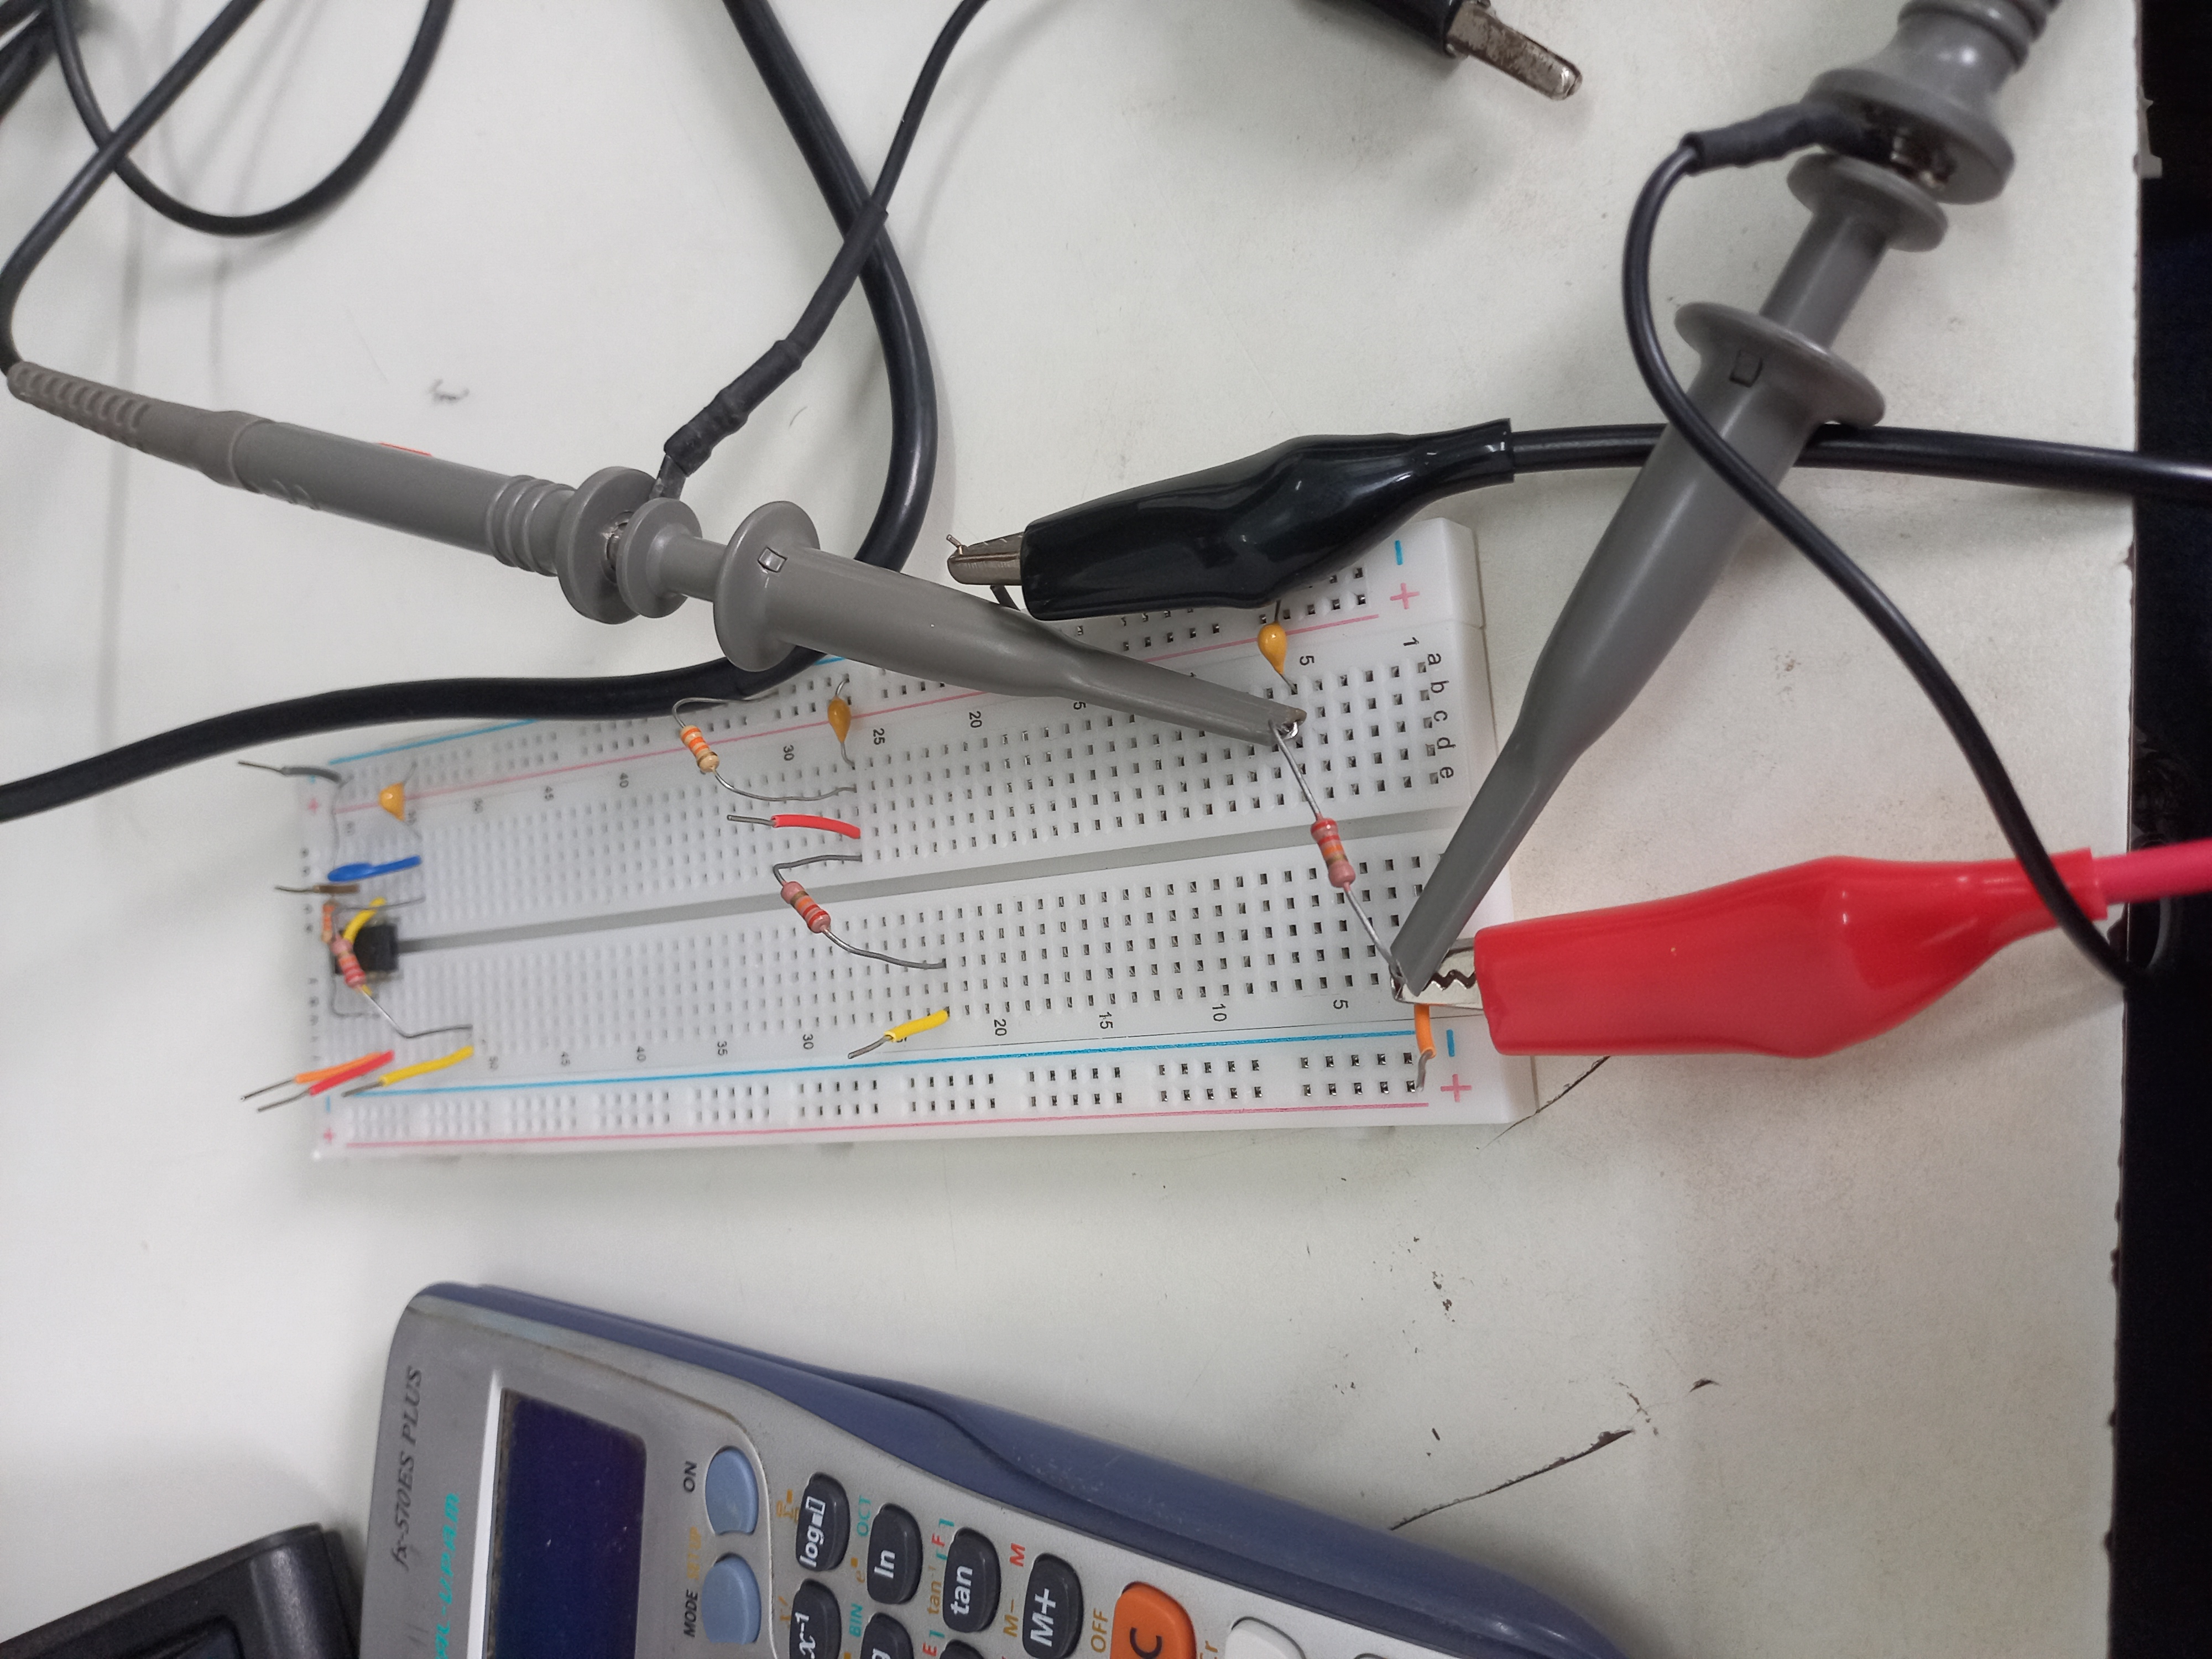
\includegraphics[width=\textwidth]{FIGURAS/circuito_montado_1.jpg}
		\caption{Montagem do Circuito 1 na \textit{protoboard}.}
		\label{fig:foto_c1}
	\end{minipage}\hfill
	\begin{minipage}{0.45\textwidth}
		\centering
		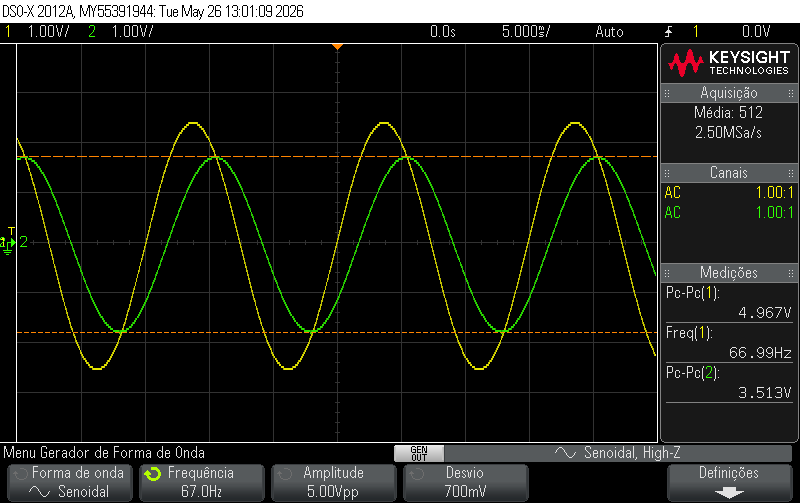
\includegraphics[width=\textwidth]{FIGURAS/67Hz_1.png} 
		\caption{Sinais $V_i$ e $V_o$ na frequência de corte ($67\text{ Hz}$).}
		\label{fig:osc_c1_fc}
	\end{minipage}
\end{figure}

\section{Circuito 2: Filtro RC com Carga Direta}

Após anexar a carga $R_L$ de aproximadamente $32\text{ k}\Omega$ em paralelo ao capacitor, o procedimento foi repetido. A nova varredura de atenuação evidenciou de forma clara o \textit{efeito de carga}, deslocando a frequência onde ocorre a queda de $3\text{ dB}$ ($V_o/V_i \approx 0,707$) para \textbf{$121\text{ Hz}$}. 

A Tabela \ref{tab:dados_c2} compila a excursão de amplitudes sobre a nova base de frequência.

\begin{table}[H]
	\centering
	\caption{Medições de amplitude em frequência para o Circuito 2 ($f_{c2} = 121\text{ Hz}$).}
	\label{tab:dados_c2}
	\renewcommand{\arraystretch}{1.2}
	\begin{tabular}{cccc}
		\hline
		\textbf{Multiplicador} & \textbf{Frequência Aplicada} & \textbf{Entrada ($V_i$)} & \textbf{Saída ($V_o$)} \\ \hline
		$0,02 \times f_{c2}$ & $2,42\text{ Hz}$ & $1,140\text{ V}$ & $460,0\text{ mV}$ \\
		$0,2 \times f_{c2}$ & $24,20\text{ Hz}$ & $4,660\text{ V}$ & $1,850\text{ V}$ \\
		$0,5 \times f_{c2}$ & $60,50\text{ Hz}$ & $5,030\text{ V}$ & $1,850\text{ V}$ \\
		$0,75 \times f_{c2}$ & $90,75\text{ Hz}$ & $5,070\text{ V}$ & $1,690\text{ V}$ \\
		$1,0 \times f_{c2}$ & $121,00\text{ Hz}$ ($f_{c2}$) & $5,100\text{ V}$ & $1,470\text{ V}$ \\
		$1,25 \times f_{c2}$ & $151,25\text{ Hz}$ & $5,110\text{ V}$ & $1,370\text{ V}$ \\
		$1,6 \times f_{c2}$ & $193,60\text{ Hz}$ & $5,110\text{ V}$ & $1,210\text{ V}$ \\
		$2,5 \times f_{c2}$ & $302,50\text{ Hz}$ & $5,110\text{ V}$ & $880,0\text{ mV}$ \\
		$3,5 \times f_{c2}$ & $423,50\text{ Hz}$ & $5,110\text{ V}$ & $680,0\text{ mV}$ \\
		$5,0 \times f_{c2}$ & $605,00\text{ Hz}$ & $5,110\text{ V}$ & $450,0\text{ mV}$ \\
		$10,0 \times f_{c2}$ & $1210,00\text{ Hz}$ & $5,110\text{ V}$ & $260,0\text{ mV}$ \\
		$20,0 \times f_{c2}$ & $2420,00\text{ Hz}$ & $5,110\text{ V}$ & $160,0\text{ mV}$ \\ \hline
	\end{tabular}
\end{table}

% Grid de fotos - Circuito 2
\begin{figure}[H]
	\centering
	\begin{minipage}{0.45\textwidth}
		\centering
		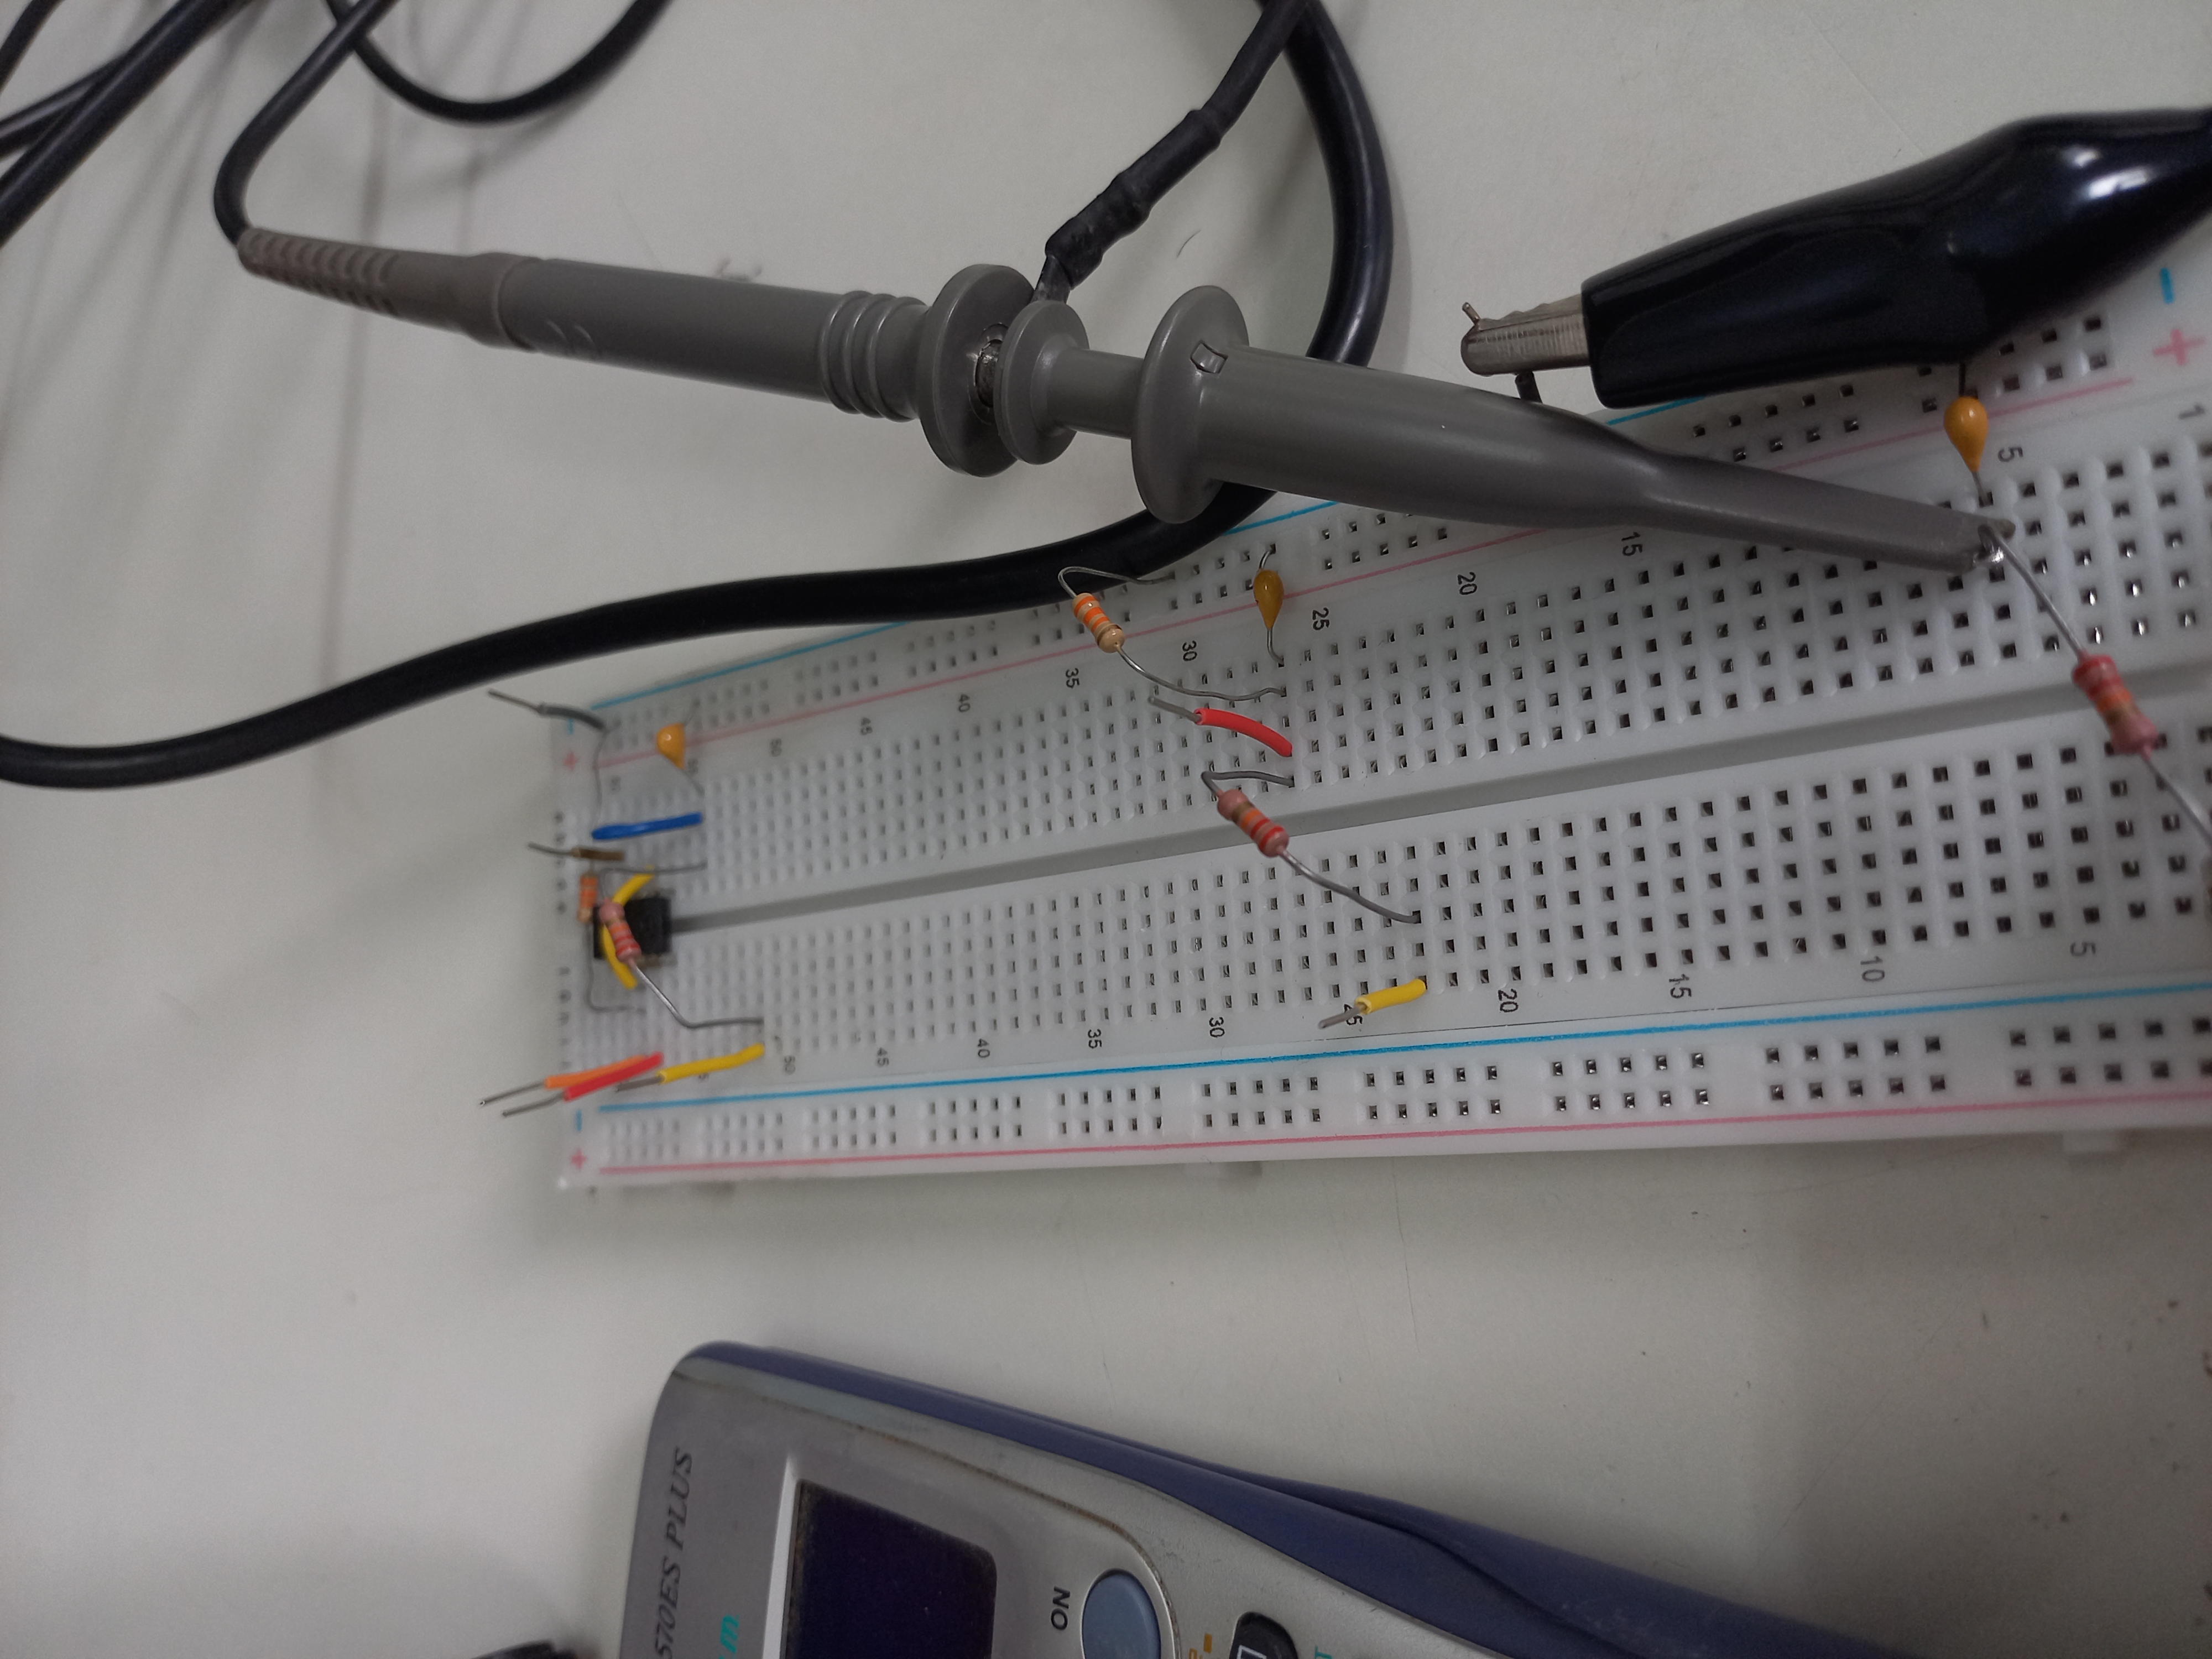
\includegraphics[width=\textwidth]{FIGURAS/circuito_2.jpg}
		\caption{Arranjo físico do Circuito 2 com resistor de carga.}
		\label{fig:foto_c2}
	\end{minipage}\hfill
	\begin{minipage}{0.45\textwidth}
		\centering
		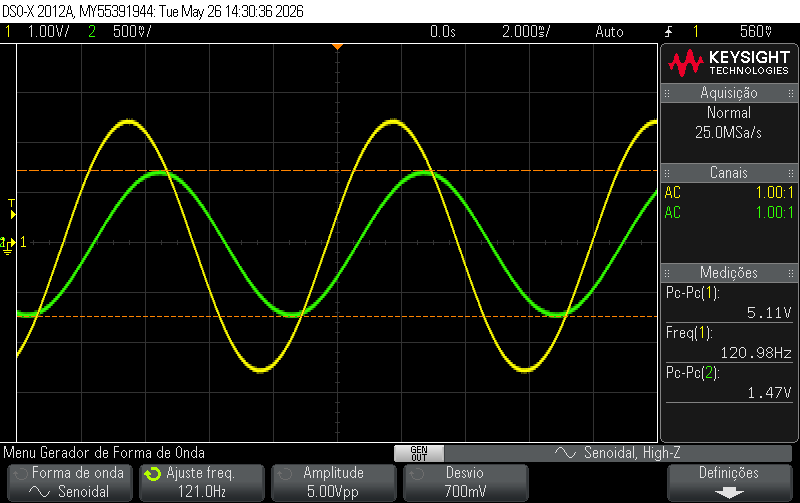
\includegraphics[width=\textwidth]{FIGURAS/121Hz_2.png} 
		\caption{Atenuação severa observada na nova frequência de corte ($121\text{ Hz}$).}
		\label{fig:osc_c2_fc}
	\end{minipage}
\end{figure}

\section{Circuito 3: Isolamento Ativo com \textit{Buffer}}

Na etapa final, introduziu-se o amplificador operacional polarizado para atuar como seguidor de tensão entre o capacitor do filtro e a resistência de carga. 

A primeira medição a $1\text{ Hz}$ registrou $V_i = 500\text{ mV}$ e $V_o = 480\text{ mV}$, comprovando que o \textit{buffer} restaurou o ganho unitário na banda de passagem ($0,96\text{ V/V}$), praticamente idêntico ao desempenho do filtro isolado original. A varredura de atenuação validou esta restauração, encontrando a nova frequência de corte em \textbf{$69\text{ Hz}$}.

Os dados colhidos para os patamares de frequência relativos a $f_{c3}$ estão reportados na Tabela \ref{tab:dados_c3}.

\begin{table}[H]
	\centering
	\caption{Medições de amplitude em frequência para o Circuito 3 ($f_{c3} = 69\text{ Hz}$).}
	\label{tab:dados_c3}
	\renewcommand{\arraystretch}{1.2}
	\begin{tabular}{cccc}
		\hline
		\textbf{Multiplicador} & \textbf{Frequência Aplicada} & \textbf{Entrada ($V_i$)} & \textbf{Saída ($V_o$)} \\ \hline
		$0,02 \times f_{c3}$ & $1,38\text{ Hz}$ & $760,0\text{ mV}$ & $760,0\text{ mV}$ \\
		$0,2 \times f_{c3}$ & $13,80\text{ Hz}$ & $3,980\text{ V}$ & $3,820\text{ V}$ \\
		$0,5 \times f_{c3}$ & $34,50\text{ Hz}$ & $4,820\text{ V}$ & $4,300\text{ V}$ \\
		$0,75 \times f_{c3}$ & $51,75\text{ Hz}$ & $4,980\text{ V}$ & $3,940\text{ V}$ \\
		$1,0 \times f_{c3}$ & $69,00\text{ Hz}$ ($f_{c3}$) & $5,030\text{ V}$ & $3,540\text{ V}$ \\
		$1,25 \times f_{c3}$ & $86,25\text{ Hz}$ & $5,070\text{ V}$ & $3,180\text{ V}$ \\
		$1,6 \times f_{c3}$ & $110,40\text{ Hz}$ & $5,110\text{ V}$ & $2,770\text{ V}$ \\
		$2,5 \times f_{c3}$ & $172,50\text{ Hz}$ & $5,110\text{ V}$ & $2,010\text{ V}$ \\
		$3,5 \times f_{c3}$ & $241,50\text{ Hz}$ & $5,110\text{ V}$ & $1,530\text{ V}$ \\
		$5,0 \times f_{c3}$ & $345,00\text{ Hz}$ & $5,110\text{ V}$ & $1,130\text{ V}$ \\
		$10,0 \times f_{c3}$ & $690,00\text{ Hz}$ & $5,110\text{ V}$ & $640,0\text{ mV}$ \\
		$20,0 \times f_{c3}$ & $1380,00\text{ Hz}$ & $5,110\text{ V}$ & $360,0\text{ mV}$ \\ \hline
	\end{tabular}
\end{table}

% Grid de fotos - Circuito 3
\begin{figure}[H]
	\centering
	\begin{minipage}{0.45\textwidth}
		\centering
		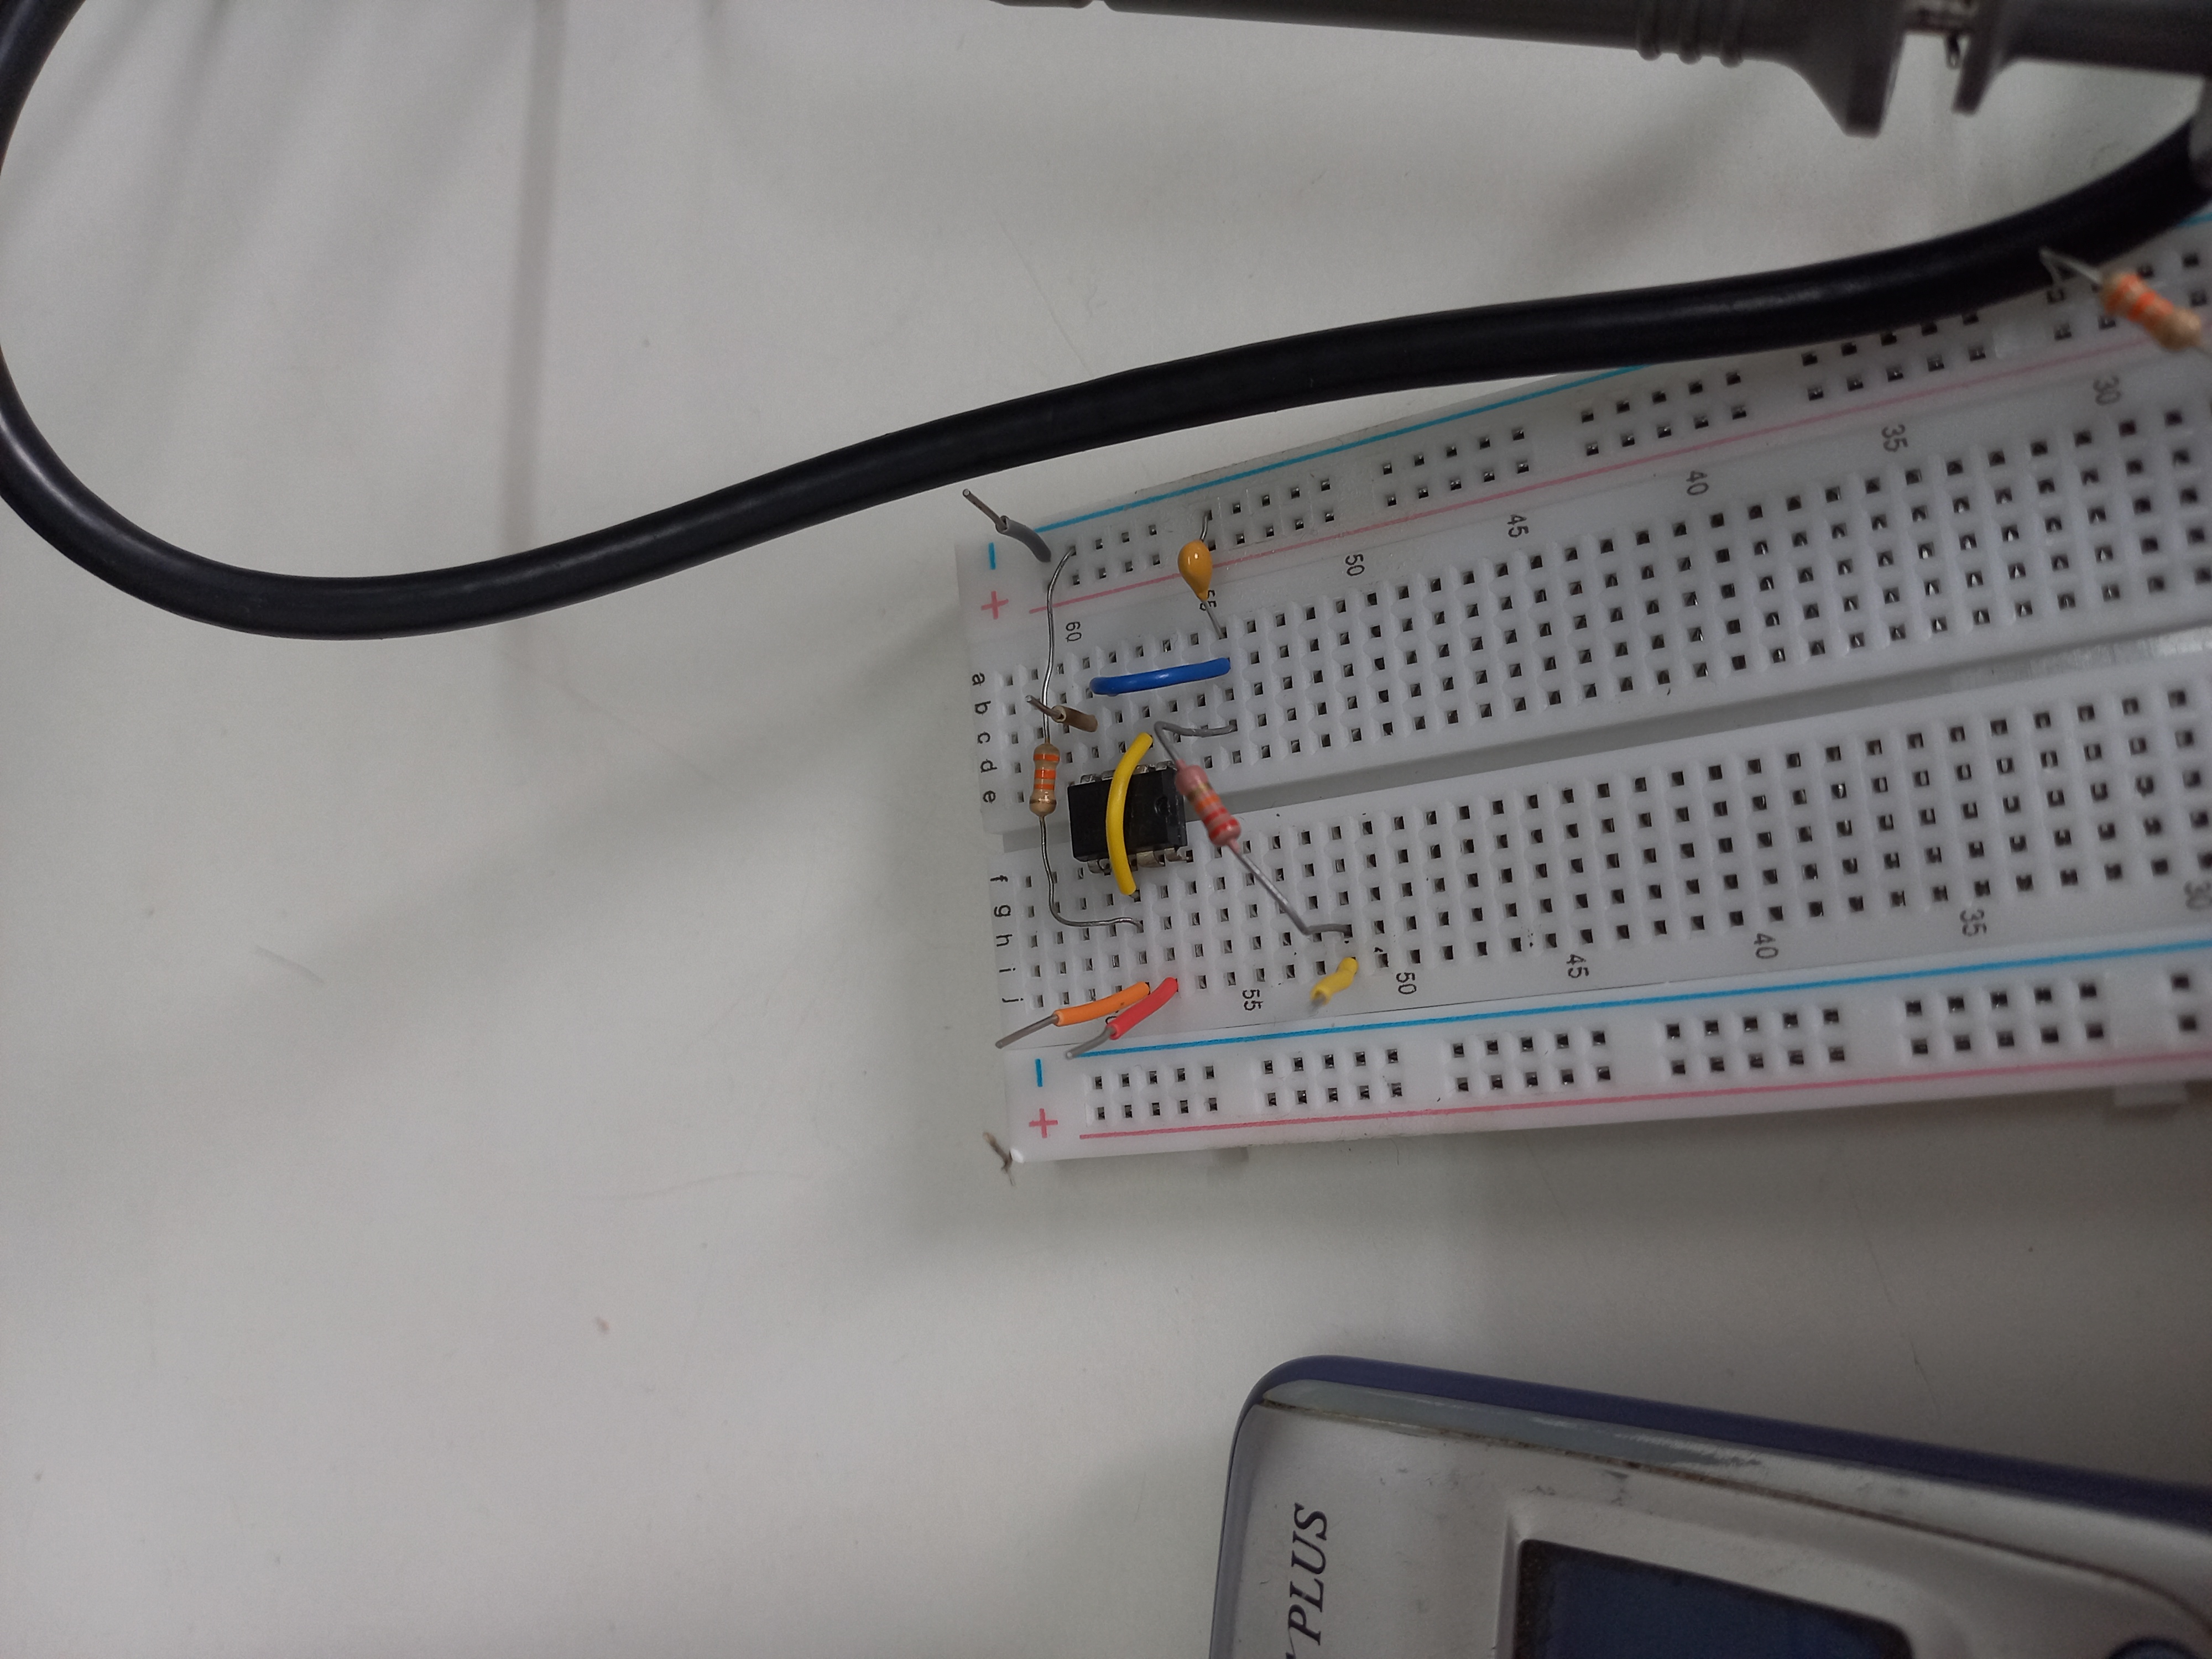
\includegraphics[width=\textwidth]{FIGURAS/circuito_3.jpg}
		\caption{Montagem completa do Circuito 3 com o ampop atuando como \textit{buffer}.}
		\label{fig:foto_c3}
	\end{minipage}\hfill
	\begin{minipage}{0.45\textwidth}
		\centering
		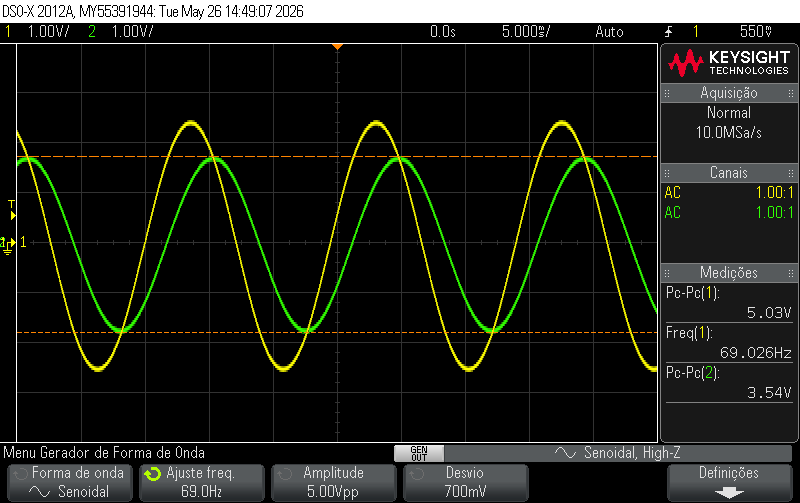
\includegraphics[width=\textwidth]{FIGURAS/69Hz_3.png} 
		\caption{Sinais estabilizados na frequência de corte restaurada ($69\text{ Hz}$).}
		\label{fig:osc_c3_fc}
	\end{minipage}
\end{figure}